\documentclass{report}

\usepackage[utf8]{inputenc}
\usepackage[T1]{fontenc}
\usepackage[francais]{babel}
\usepackage{lmodern}
\usepackage{graphicx, subfigure}
\usepackage{amsmath}
\usepackage{amssymb}
\usepackage{mathrsfs}
\usepackage{geometry}
\geometry{scale=0.8, nohead}

\author{Nicolas Ehrhardt et David Hoffmann}
\title{Compression d'image et triangulation}

\makeatletter
\renewcommand{\thesection}{\@arabic\c@section}
\makeatother

\begin{document}
\maketitle
\section{Introduction}

La compression d'image est dominée par des algorithmes basés sur les transformées de Fourier et plus récemment sur la théorie des ondelettes. L'un des désavantages souvent critiqué de la compression par stockage des coefficients de Fourier est son caractère non-localisant. La théorie des ondelettes se propose de résoudre ce problème.

Si la théorie de Fourier est valable pour tout type de signal elle ne prend pas assez en compte le caractère ordonné d'une image. En effet, les objets dans l'image ont une structure particulière : des bords et des surfaces homogènes notamment. Pour mieux rendre compte de cette structure interne, un nouveau type de compression a été introduit, il consiste à stocker un nombre de points fixés de l'image avec leur couleur sous forme de matrice creuse, ainsi qu'une triangulation associée.

\subsection{Décompression d'une triangulation}

On obtient alors l'image décodée de manière suivante. Pour tout point de l'image, chercher le triangle de la triangulation qui le contient, obtenir alors ses coordonnées barycentriques $x_1, x_2, x_3$ associées aux trois sommets du triangle. On note dans le même ordre $c_1, c_2, c_3$ les couleurs des trois sommets. La couleur du point en question est alors $\sum x_i c_i$.

Il est assez simple de voir que l'image reconstruite sera alors composée de triangles dans lesquels la couleur sera un dégradé entre les sommets. Ainsi, on s'attend à avoir une image lissée en quelque sorte et non pas "bruitée" dans le cas d'une compression type Fourier de mauvaise qualité.

\subsection{Erreur}

Plusieurs types d'erreurs peuvent être utilisés pour comparer les qualités des images. Considérons notre image comme une surface, pour chaque pixel, sa couleur (coordonnée $z$) est fonction de son abscisse et de son ordonnée dans dans l'image ($x, y$). On notera $c(x, y) = I(x, y)$ l'image originale, et $c_d(x, y) = I_d(x, y)$ l'image décompressée.

\subsubsection{Erreur $L^p$}

Comme indiqué, il suffit de calculer la quantité suivante pour obtenir l'erreur $L^p$ :

$$ (\sum_x \sum_y \vert c(x,y) - c_d(x, y) \vert^p )^{\frac{1}{p}} $$

Ceci étant généralisable à $L^\infty$.

\subsubsection{Erreur $L^p$ en projection}

Pour cette erreur, il s'agit de projeter tout point de l'image $I$ sur l'image $I_d$. Dans notre cas, puisque l'image décompressée est une union de triangles on considère la distance au plan associé au triangle.

$$ (\sum_x \sum_y \vert \pi_d c(x,y) - c_d(x, y) \vert^p )^{\frac{1}{p}} $$

Cette erreur est contestable nous en ferons la démonstration.

\section{Algorithme de compression adaptatif}

Si s'intéresser à une triangulation a des avantages sur le plan visuel, il en a aussi sur le plan théorique. On a vu en introduction que l'on stockait les points sous forme de matrice sparse pour gagner en place, mais cela ne nous affranchi pas du stockage de la triangulation, sous forme d'une matrice $n \times 3$. Hormis si l'on travaille avec une triangulation de Delaunay... Évidemment, cette triangulation étant unique, il est inutile de la stocker, elle peut très bien être reconstruite juste avant la décompression en $O(N ln(N))$.

\subsection{Principe de l'algorithme}

\paragraph{Initialisation :}

On construit un maillage qui inclut tous les points de l'image ($N$). Chaque point ayant comme erreur associée la couleur maximale de ses quatres voisins moins la couleur minimale de ses quatre voisins.

\paragraph{Étape i :}

On dispose de $N-i$ points dans notre maillage.
On choisit le point auquel est associé la plus petite erreur et on l'enlève du maillage.
On recalcule la triangulation de delaunay pour ses points voisins.
Et on met à jour leur erreur associée.

\paragraph{Critère d'arrêt :}
On peut se donner un nombre de points à enlever, ou demander à s'arrêter lorsque l'erreur atteint un seuil.

\paragraph{Calcul de l'erreur associée :}
L'erreur associée à un point est l'erreur entre l'image décompressée à partir du maillage auquel on aurait enlevé ce point et l'image initiale. Celle-ci dépend du choix de la méthode avec laquelle nous calculerons l'erreur.

\subsection{Résultats}

Prenons pour commencer une image avec un certain nombre de bords et de la texture. Comme d'habitude, notre amie Lena fera parfaitement l'affaire. Il faudra regarder de plus près les cheveux et le haut du chapeau pour voir apparaître les premières erreurs.

\begin{figure}[ht!]
     \begin{center}
        \subfigure[Image originale]{%
            \label{fig:first}
            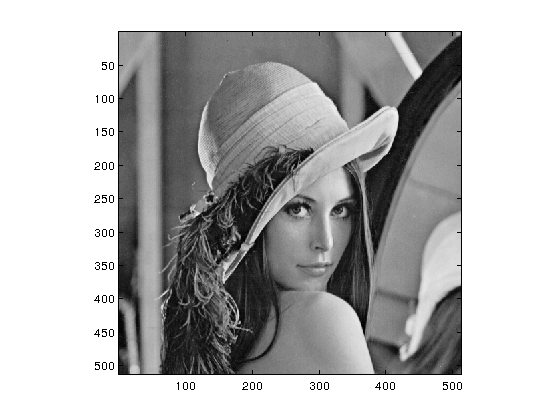
\includegraphics[width=0.5\textwidth]{lena.png}
        }%
        \subfigure[102144 Noeuds; snr : 3.4489]{%
           \label{fig:second}
           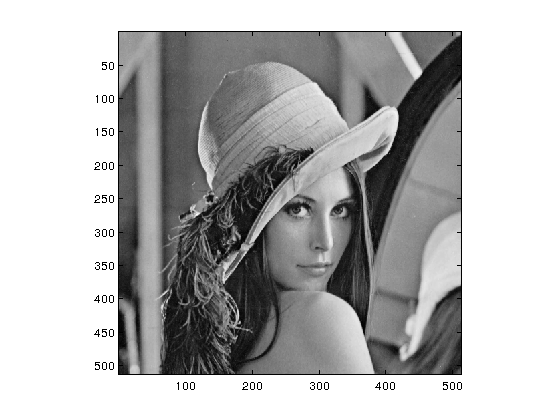
\includegraphics[width=0.5\textwidth]{lenaDelau100000.png}
        }\\ %  ------- End of the first row ----------------------%
        \subfigure[42144 Noeuds; snr : 9.9287]{%
            \label{fig:third}
            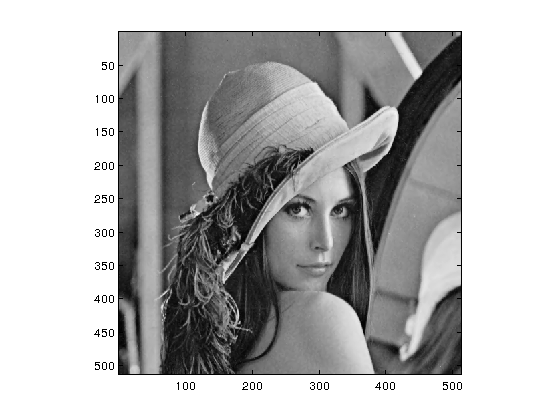
\includegraphics[width=0.5\textwidth]{lenaDelau40000.png}
        }%
        \subfigure[12144 Noeuds; snr : 25.9734]{%
            \label{fig:fourth}
            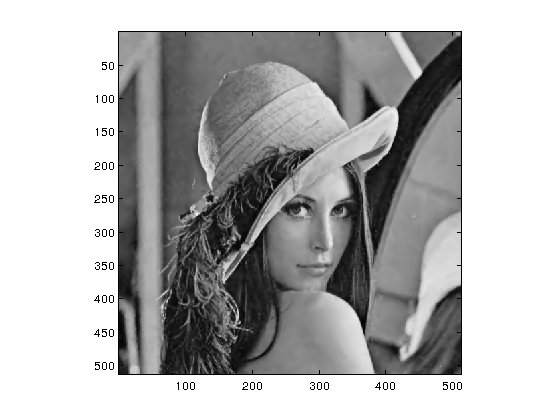
\includegraphics[width=0.5\textwidth]{lenaDelau10000.png}
        }\\ %  ------- End of the first row ----------------------%
        \subfigure[7144 Noeuds; snr : 39.5056]{%
            \label{fig:fifth}
            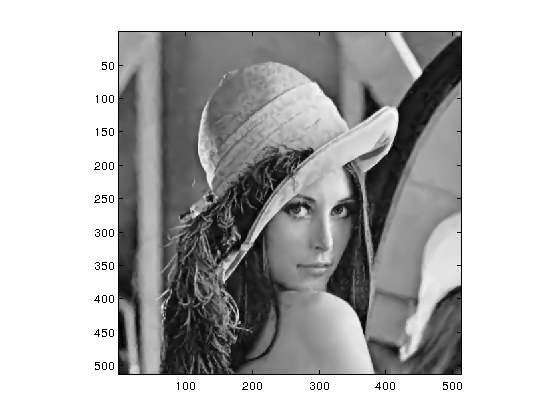
\includegraphics[width=0.5\textwidth]{lenaDelau7000.png}
        }%
        \subfigure[4144 Noeuds; snr : 63.0030]{%
            \label{fig:sixth}
            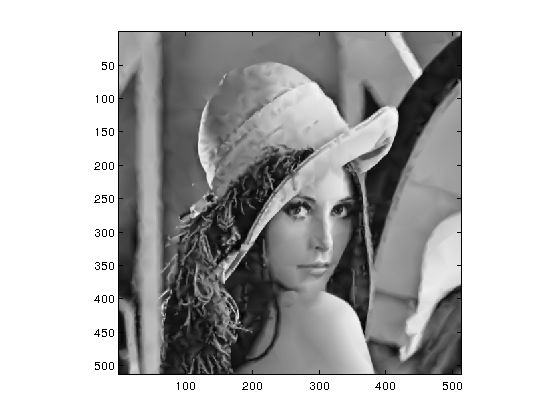
\includegraphics[width=0.5\textwidth]{lenaDelau4000.png}
        }%    
    \end{center}
    \caption{%
        Résultat pour l'algorithme de compression adaptatif
    }%
   \label{fig:subfigures}
\end{figure}


\section{Algorithme des bissections}

\subsection{Principe}


\subsection{Description de l'algorithme}

\paragraph{Initialisation :}

On part d'un maillage minimal avec les 4 coins et 2 triangles, comme sur la figure :

///////////
  SCHEMA
Triangulation initiale
///////////

\paragraph{Étape i :}

On commence par chercher parmi tous les triangles quel est celui qui porte la plus grande erreur d'approximation, pour le couper en deux. Une fois ce triangle choisi, on doit déterminer quelle est la meilleure manière de le couper. En pratique, on s'autorise 3 coupes possibles, qui correspondent aux 3 médianes du triangle choisi :

///////////
  SCHEMA
Médianes d'un triangle
///////////

On détermine parmi ces 3 médianes laquelle est la coupe la plus avantageuse. Puis on effectue la coupe, autrement dit :
\begin{itemize}
	\item - On ajoute un point (le sommet de la médiane qu'on doit créer)
	\item - On enlève de la triangulation le triangle sur lequel on travaillait
	\item - On ajoute à la place les deux triangles issus de la coupe
\end{itemize}

///////////
  SCHEMA
Coupe selon une médiane
///////////



\paragraph{Critère d'arrêt :}
On peut se donner un nombre de point à enlever, ou demander à s'arrêter lorsque l'erreur atteint un seuil.

\paragraph{Calcul de l'erreur associée :}
L'erreur associée à un point est l'erreur entre l'image décompressée à partir du maillage auquel on aurait enlevé ce point et l'image initiale. Celle-ci dépend du choix de la méthode avec laquelle nous calculerons l'erreur.

\subsection{Résultats}

Prenons pour commencer une image avec un certain nombre de bords et de la texture. Comme d'habitude, notre amie Lena fera parfaitement l'affaire. Il faudra regarder de plus près les cheveux et le haut du chapeau pour voir apparaître les premières erreurs.
\end{document}
